\chapter{Literature Review}
\label{ch:literature}

\section{BasePaper I: Heged\H{u}s and Ferenc (2022)}
\label{sec:bp1}

\textbf{P.\ Heged\H{u}s and R.\ Ferenc, ``Static Code Analysis Alarms Filtering
Reloaded: A New Real-World Dataset and Its ML-Based Utilization,'' \textit{IEEE
Access}, vol.~10, 2022.} \cite{hegedus2022sca}

This paper is the primary methodological reference for the present project.
The authors identify three pervasive limitations in prior SCA false-positive
filtering research: (i)~approaches target only a small subset of warning types;
(ii) evaluations use synthetic or small benchmarks; (iii) datasets are closed and
non-replicable. They address all three by mining GitHub history to construct a
dataset of \textbf{224,484 real-world SonarQube warnings} from 9,958 Java
projects, labelled using explicit developer actions (fix commit = true positive;
\texttt{//NOSONAR} = false positive). The data covers 160 SonarQube rule checks.

The classification pipeline consists of:
\begin{enumerate}
  \item \textbf{Feature extraction}: the warning line and $n$~surrounding lines
        are tokenized using the \texttt{javalang} lexer.
  \item \textbf{Code embedding}: tokens are embedded with word2vec
        (64-dimensional vectors, window~5) trained on 0.5M Java files.
  \item \textbf{Classification}: four ML classifiers are evaluated ---
        Decision Tree (DTree), Naive Bayes (NBayes), Random Forest (RForest),
        Neural Network (NeuralNet) --- using 10-fold cross-validation with
        stratified sampling per SonarQube warning type and upsampling for
        class imbalance.
\end{enumerate}

\begin{figure}[htbp]
  \centering
  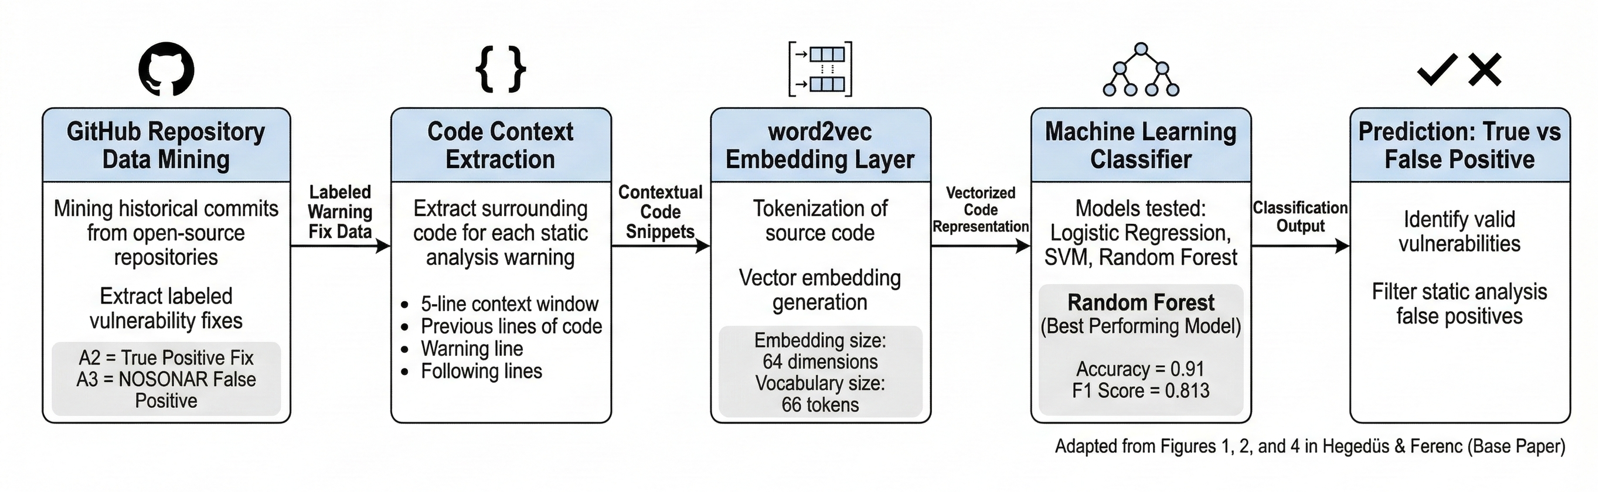
\includegraphics[width=0.9\textwidth]{Figures/fig_bp1_pipeline.png}
  \caption{Classification pipeline of BasePaper~I \cite{hegedus2022sca}. Real-world
           SonarQube warnings are labelled via developer actions, embedded with
           word2vec, and classified by an ensemble model.}
  \label{fig:bp1_pipeline}
\end{figure}

\textbf{Key results:} Random Forest achieves accuracy~=~0.91, precision~=~0.874,
recall~=~0.760, F1~=~0.813, AUC~=~0.953 on 224,484 real-world warnings across
160 SonarQube rule types. The model correctly filters out 76\% of false positive
warnings while misclassifying only 8\% of true positives as false, preserving
developer attention for real issues.

\textbf{Relevance to this project:} This work directly motivates the use of a
Random Forest classifier for SARIF alert triage in our pipeline. The code-context
embedding strategy and word2vec representation are adapted for our feature set.

\section{BasePaper II: Syed et al.\ (2025)}
\label{sec:bp2}

\textbf{T.A.\ Syed et al., ``Agentic AI for Autonomous Defense in Software Supply
Chain Security: Beyond Provenance to Vulnerability Mitigation,'' arXiv:2512.23480,
2025.} \cite{syed2025agentic}

Syed et al.\ present a multi-agent agentic AI framework for autonomous software
supply chain security. Five specialised agents (Code Analysis, Dependency
Intelligence, CI/CD Monitoring, Access Control, Configuration Audit) are
orchestrated by LangChain and LangGraph. LLM semantic reasoning and PPO-based RL
policies drive mitigation decisions; all agent actions are recorded in a
permissioned blockchain ledger; CI/CD integration is achieved via the Model Context
Protocol (MCP). The framework achieves F1-scores above 0.93 across four
vulnerability classes and reduces mean time-to-mitigation from 28~min to
$<$6~min compared to rule-based systems.

\textbf{Relevance:} Provides the agentic AI design principles (perceive--reason
--act--learn loop, LangGraph conditional routing, LLM chain-of-thought reasoning)
that inform the agentic triage and remediation layer of the present system.

\section{Third Reference: Charoenwet et al.\ (2026)}
\label{sec:3rd}

\textbf{W.\ Charoenwet et al., ``AgenticSCR: An Autonomous Agentic Secure Code
Review for Immature Vulnerabilities Detection,'' arXiv:2601.19138, 2026.}
\cite{charoenwet2026agenticscr}

AgenticSCR is an agentic framework for pre-commit vulnerability detection using a
detector--validator subagent pair. The detector subagent loads SAST rules as
long-term semantic memory; the validator cross-checks findings against a CWE
knowledge tree. Evaluated on SCRBench (144 pre-commit changes, 33 CWE types),
it achieves 17.5\% overall correct comments --- 153\% higher than a static LLM
baseline --- while generating 2--5$\times$ fewer comments.

\textbf{Relevance:} The detector--validator pattern motivates the pipeline design
where the ML classifier (detector) and agentic triage layer (validator) are
distinct but complementary stages. The use of SAST rules as semantic memory
informs feature design.

\section{Fourth Reference: Bakane (2025)}
\label{sec:4th}

\textbf{S.\ Bakane, ``Agentic AI for Autonomous Risk Triage and False Positive
Reduction in Static Security Analysis,'' M.Sc.\ Thesis, University of Turku, 2025.}
\cite{bakane2025thesis}

Bakane proposes an agentic AI pipeline that normalises heterogeneous outputs of
GitLeaks, OWASP Dependency-Check, and Semgrep into a unified schema and applies
rule-based heuristics combined with LLM reasoning to triage alerts. The system
achieves a 31\% false positive reduction and produces dashboards compliant with
OWASP SAMM, BSIMM, and NIST SSDF.

\textbf{Relevance:} The normalisation layer (unified schema from heterogeneous tool
outputs) and compliance reporting directly inform the output design and evaluation
criteria of the present pipeline's agentic triage component.

\section{Synthesis}

Table~\ref{tab:litreview} positions all four references in terms of their stage in
the vulnerability management lifecycle. Together they form a coherent rationale for
the present project: ML-based alert filtering (BasePaper~I) augmented by agentic AI
reasoning following the principles of BasePaper~II, 3rd, and 4th.

\begin{table}[htbp]
  \centering
  \caption{Summary and Positioning of Primary References}
  \label{tab:litreview}
  \renewcommand{\arraystretch}{1.35}
  \begin{tabular}{p{3cm}p{2.5cm}p{4cm}p{2.5cm}}
    \toprule
    \textbf{Reference} & \textbf{Stage} &
    \textbf{Key Contribution} & \textbf{Gap Remaining} \\
    \midrule
    Heged\H{u}s \& Ferenc \cite{hegedus2022sca} &
      Post-scan alert triage &
      224K real-world labelled SonarQube warnings; RForest 91\% accuracy &
      Static dataset; no agentic remediation \\
    Syed et al.\ \cite{syed2025agentic} &
      Supply chain defense &
      Multi-agent LLM+RL framework with MCP and blockchain &
      No ML-based alert filtering \\
    Charoenwet et al.\ \cite{charoenwet2026agenticscr} &
      Pre-commit review &
      Detector--validator subagents; 153\% improvement over static LLM &
      No ML triage \\
    Bakane \cite{bakane2025thesis} &
      Static output triage &
      31\% false positive reduction; OWASP SAMM/NIST SSDF compliance &
      No commit-level integration \\
    \bottomrule
  \end{tabular}
\end{table}
